\section{Data Distribution and Preprocessing}
\label{sec:data}
\subsection{Statlog German Credit Data}

\textbf{Provenance and licence.} We use the Statlog German Credit data
(\texttt{credit-g})~\cite{uci_credit_g_1994}, donated by Hans Hofmann (University of
Hamburg, 1994) to the UCI Machine Learning Repository~\cite{dua2019uci} (UCI ID~144,
DOI 10.24432/C5NC77). The dataset is released under the CC BY 4.0 licence and is
cited accordingly.

\textbf{Attribute schema.} The dataset contains 1{,}000 applicants $\times$ 21
columns: 13 nominal attributes, 7 numeric attributes and the binary target
\texttt{class} (\texttt{good} vs.\ \texttt{bad}; the positive class is \texttt{bad}
throughout this report). The full 21-row dictionary with business semantics, value
sets and per-column missing counts is archived as
\texttt{results/credit-g\_schema.xlsx}.

\textbf{Class distribution and data quality.} Figure~\ref{fig:a_class} shows the
class distribution: 700 \texttt{good} versus 300 \texttt{bad}, i.e., a 30\%
positive rate and a moderate 70:30 imbalance. A systematic quality audit reports
zero missing values and zero duplicated rows across all 21 columns, so
\texttt{credit-g} requires no imputation and no row or column deletion. The 70:30
ratio also fixes the reference points used later: a majority-class baseline already
scores 0.70 accuracy (revisited in Section~\ref{sec:results}), and all resampling
and cost-sensitive strategies are motivated by this imbalance.

% Source: figures/fig_a_class.png = figures/fig1_class_distribution.png (src/a4_creditg_eda.py)
\begin{figure}[H]
\centering
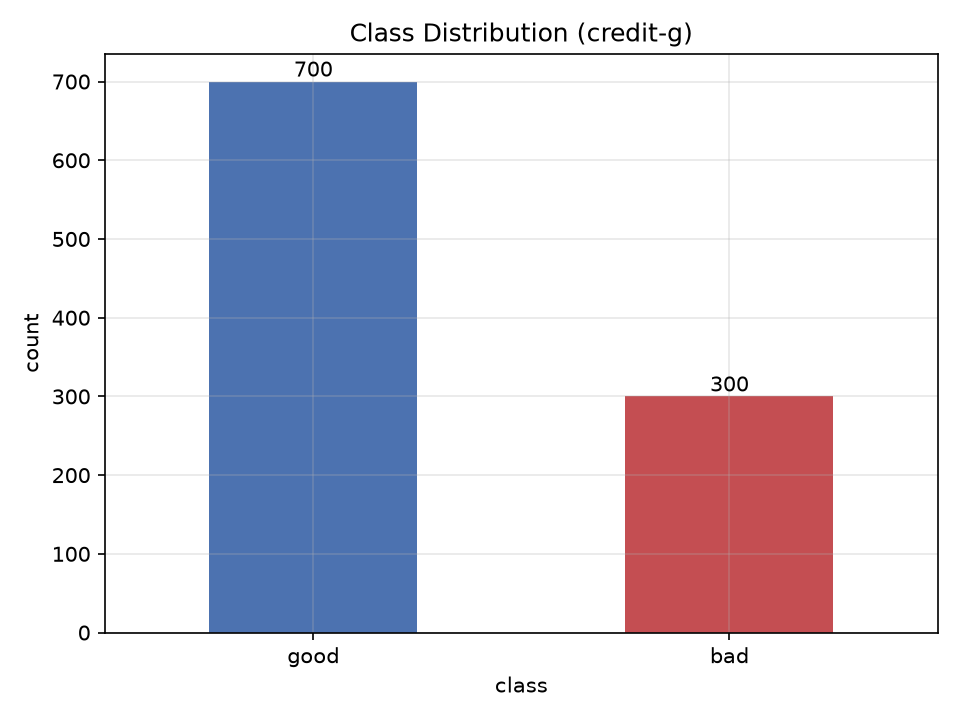
\includegraphics[width=0.55\textwidth]{figures/fig_a_class.png}
\caption{Class distribution of \texttt{credit-g} (1{,}000 records; positive class
= \texttt{bad}): 700 \texttt{good} vs.\ 300 \texttt{bad} (30\% positive rate), a
70:30 class imbalance. Source: \texttt{figures/fig1\_class\_distribution.png}
(\texttt{src/a4\_creditg\_eda.py}).}
\label{fig:a_class}
\end{figure}

\textbf{Descriptive statistics.} Of the seven numeric attributes, three are
genuinely continuous (\texttt{duration}, \texttt{credit\_amount}, \texttt{age}) and
four are ordinal grade fields on 1--4 or 1--2 scales. Figure~\ref{fig:a_numeric}
shows that all three continuous attributes are right-skewed --- for
\texttt{credit\_amount} the median (2{,}320 DM) lies far below the mean (3{,}271 DM)
and the maximum (18{,}424 DM) --- a skew that directly informs the discretisation
choice below.

% Source: figures/fig_a_numeric.png = figures/fig3_numeric_hist.png (src/a4_creditg_eda.py)
\begin{figure}[H]
\centering
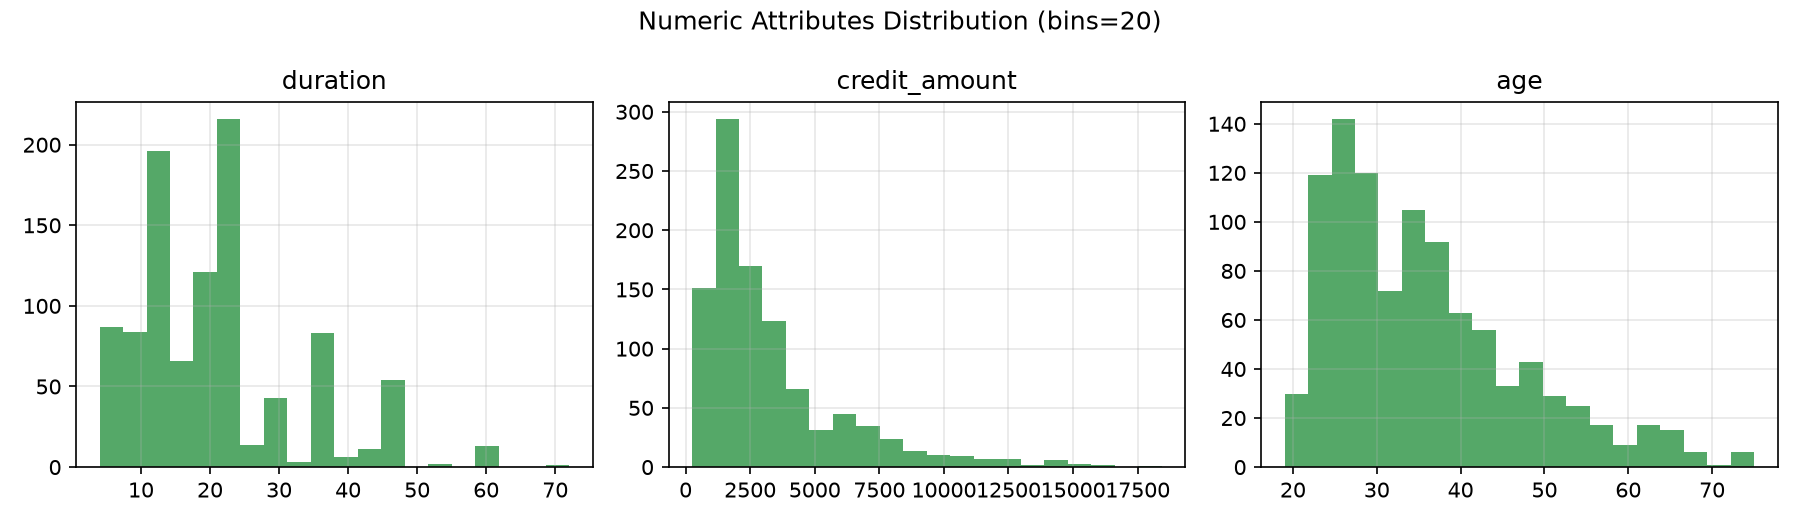
\includegraphics[width=0.95\textwidth]{figures/fig_a_numeric.png}
\caption{Histograms (bins = 20) of \texttt{duration}, \texttt{credit\_amount} and
\texttt{age} in \texttt{credit-g}; all three are right-skewed, with
\texttt{credit\_amount} ranging from 250 to 18{,}424 DM. Source:
\texttt{figures/fig3\_numeric\_hist.png} (\texttt{src/a4\_creditg\_eda.py}).}
\label{fig:a_numeric}
\end{figure}

Among the nominal attributes, \texttt{checking\_status} shows the clearest
relationship with the target. Figure~\ref{fig:a_checking} sorts its four values by
default rate: the \texttt{bad} share falls monotonically from 49.3\% (overdrawn
accounts, \texttt{<0}, 135 of 274) to 39.0\% (\texttt{0<=X<200}), 22.2\%
(\texttt{>=200}) and 11.7\% (no checking account, 46 of 394), straddling the 30\%
overall rate. This gradient is consistent with domain intuition (weaker account
standing, higher default risk) and is later corroborated by tree-based feature
importances in the interpretability analysis.

% Source: figures/fig_a_checking.png = figures/fig2_checking_status_class.png (src/a4_creditg_eda.py)
\begin{figure}[H]
\centering
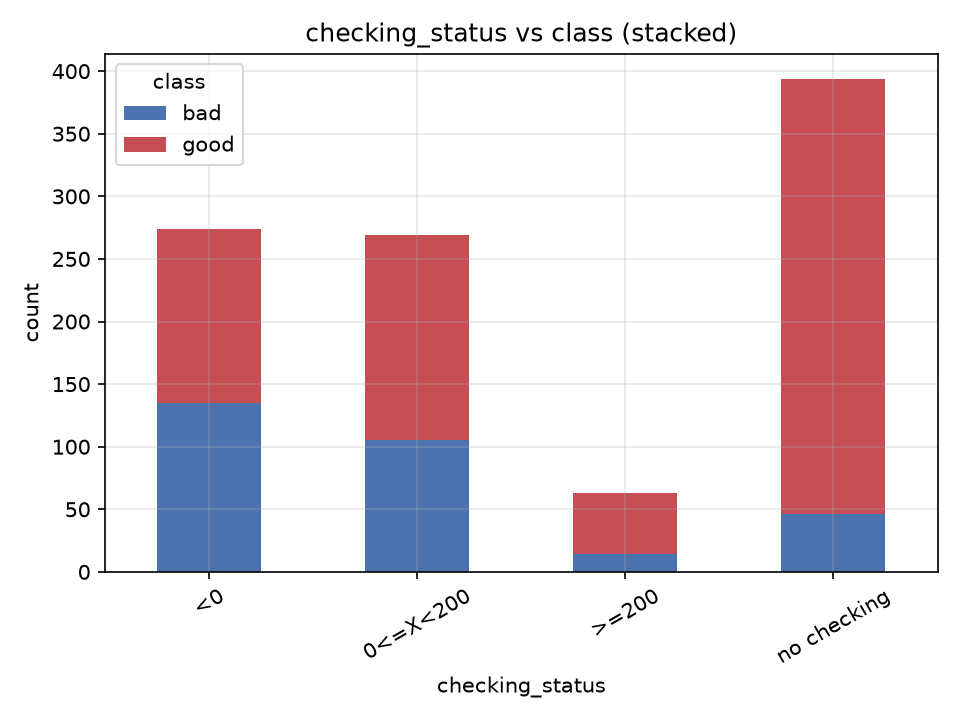
\includegraphics[width=0.72\textwidth]{figures/fig_a_checking.png}
\caption{Stacked class distribution by \texttt{checking\_status} in \texttt{credit-g},
sorted by default rate (positive class = \texttt{bad}). Overdrawn accounts
(\texttt{<0}) show the highest \texttt{bad} rate (49.3\%), accounts without a
checking account the lowest (11.7\%). Source:
\texttt{figures/fig2\_checking\_status\_class.png}
(\texttt{src/a4\_creditg\_eda.py}).}
\label{fig:a_checking}
\end{figure}

\textbf{Preprocessing decisions.} Four preprocessing decisions are adopted for
\texttt{credit-g}:
\begin{enumerate}
  \item \emph{No cleaning.} The quality audit (0 missing, 0 duplicated) removes the
  need for imputation or deletion; the raw table enters the pipelines unchanged.
  \item \emph{Linear and kernel models} (logistic regression, RBF-SVM) receive the
  13 nominal attributes one-hot encoded (\texttt{handle\_unknown='ignore'}) and the
  numeric attributes standardised to zero mean and unit variance.
  \item \emph{Tree-based models} (decision tree, random forest) receive ordinal
  codes for the nominal attributes (\texttt{unknown} $\rightarrow$ $-1$) and
  unscaled numerics: tree splits depend on orderings and thresholds only, so
  one-hot expansion would merely dilute split gains and scaling has no effect.
  \item \emph{Discretisation for association analysis}: the continuous attributes
  \texttt{duration}, \texttt{credit\_amount} and \texttt{age} are binned with
  \texttt{KBinsDiscretizer} into five \emph{quantile} bins, and nominal values are
  used as items directly (Section~\ref{sec:apriori}). Quantile bins rather than
  equal-width bins are used precisely because the right skew of
  Figure~\ref{fig:a_numeric} would collapse most records into the lowest equal-width
  bin.
\end{enumerate}

A controlled ablation confirms the branch assignment of decisions 2 and 3 (RQ3).
Table~\ref{tab:a_encoding} compares logistic regression under the two encodings by
stratified 10-fold cross-validation (seed 42; positive class \texttt{bad}): one-hot
encoding with standardised numerics outperforms ordinal encoding with raw numerics
on every metric, and the gains in F1 and ROC-AUC are statistically significant
under fold-level paired $t$-tests ($n = 10$, uncorrected). One-hot encoding with
standardised numerics is therefore used for all linear/kernel models and ordinal
codes with raw numerics for all tree-based models throughout the main matrix. Full
fold-level results are archived in \texttt{results/a6\_onehot\_comparison.csv} and
\texttt{results/a6\_onehot\_folds.csv}.

\begin{table}[H]
\centering
\caption{Encoding ablation on \texttt{credit-g} (logistic regression, stratified
10-fold CV, seed 42, positive class = \texttt{bad}; means over $n = 10$ folds).
Source: \texttt{results/a6\_onehot\_comparison.csv}.}
\label{tab:a_encoding}
\begin{tabular}{lrrrr}
\toprule
Encoding & Features & Accuracy & F1 (\texttt{bad}) & ROC-AUC \\
\midrule
One-hot + standardised numerics & 61 & \textbf{0.752} & \textbf{0.531} & \textbf{0.785} \\
Ordinal + raw numerics & 20 & 0.718 & 0.406 & 0.738 \\
\midrule
Paired $t$-test $p$ ($n = 10$ folds) & --- & 0.101 & 0.021 & 0.008 \\
\bottomrule
\end{tabular}
\end{table}
